\chapter{Estado de la Cuestión}
\label{cap:estadoDeLaCuestion}
En este capítulo se presenta una breve descripción del desarrollo de las simulaciones físicas en videojuegos, así como el hardware y software que ha hecho que esta evolución sea posible, se presenta la simulación de telas en específico, las maneras que existen de implementarla, los problamas de optimización que estas suponen y los avances en modelos de IA que permiten imaginar otras soluciones.

\section{Simulación física en videojuegos}
Como se puede ver en el artículo \cite{XGKD23}, se empezó a hablar en la década\dots
Contexto histórico de simulaciones físicas en videojuegos, 
prerender
obj únicos
coherencia: lo que se busca ahora (hiperrealismo tal) utilizo para justificar sistemas unidos d fisicas y las maneras d hacer esto:

\subsection{Motores físicos}
PHYSIS HAVOC BULLET
intereses por trabajar cn la CPU vs GPU

\subsection{Motores de videojuegos}
estos usan physis: hoy en día unreal y UNITY (justificamos por qué unity: libre acceso, motor principal usado para desarrollo?)

Unity es un motor de videojuegos creado por Unity Technologies en 2005. Su motor físico: PhysX, creado por la empresa Nvidia Corporation.
Unreal es un motor de videojuegos creado por Epic Games en 1998 con el lanzamiento de Unreal Engine 1.
La versión estable actual es Unreal Engine 5.5, lanzada en noviembre de 2024.
El código fuente de este motor está escrito en C++ y es accesible desde Github \footnote{Enlace a la página de Github de Epic: \url{https://github.com/epicgames}}.
Usa PhysX igualmente asi q txau.

\subsection{Simulación de telas}
Los distintos tipos de simulaciones que se implementan en los motores de físicas previamente mencionados, podrían agruparse en los siguientes grupos: Collision detection,ragdoll physics, particle systems (fluids y fuzzy), deformable bodies (entre ellos rigid-bodies y soft-bodies). En concreto soft-bodies / cloth. EVA DALE.

\begin{figure}[H]
    \centering
    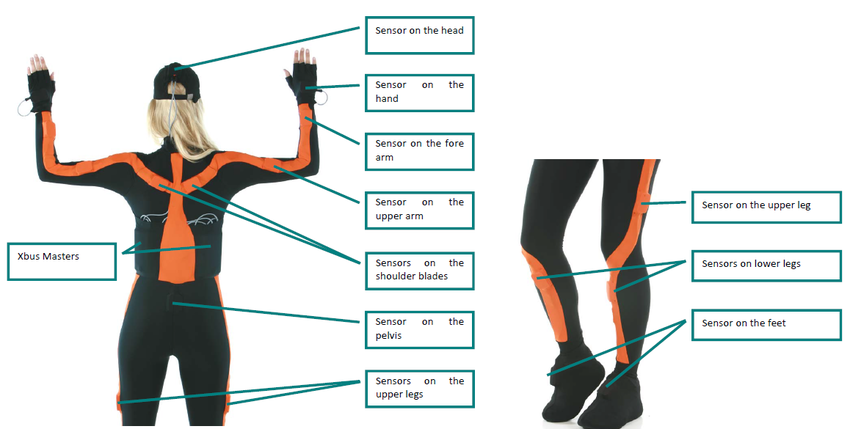
\includegraphics[width=0.5\textwidth]{Imagenes/Bitmap/XSens.png}
    \caption[Imágen del traje de captura de movimiento XSens]{Imágen del traje de captura de movimiento XSens \footnotemark }
    \label{fig:XSensTraje}
\end{figure}

\footnotetext{Fuente de la imagen: \url{https://www.researchgate.net/figure/The-Xsens-MVN-full-body-motion-capture-suit-Picture-source-htttp-wwwxsenscom_fig1_233926874}}